\chapter{Экспериментальный раздел}
\label{cha:research}

В данном разделе будут приведены примеры работы разработанного
приложения и поставлен эксперимент по сравнению производительности
в зависимости от сложности моделируемой сцены. Сложность оценивается количеством используемых на сцене поверхностей.

\section{Результаты работы программного обеспечения}
На рисунке \ref{fig:example_run} изображен пример выполнения программы. 
\begin{figure}
  \centering
  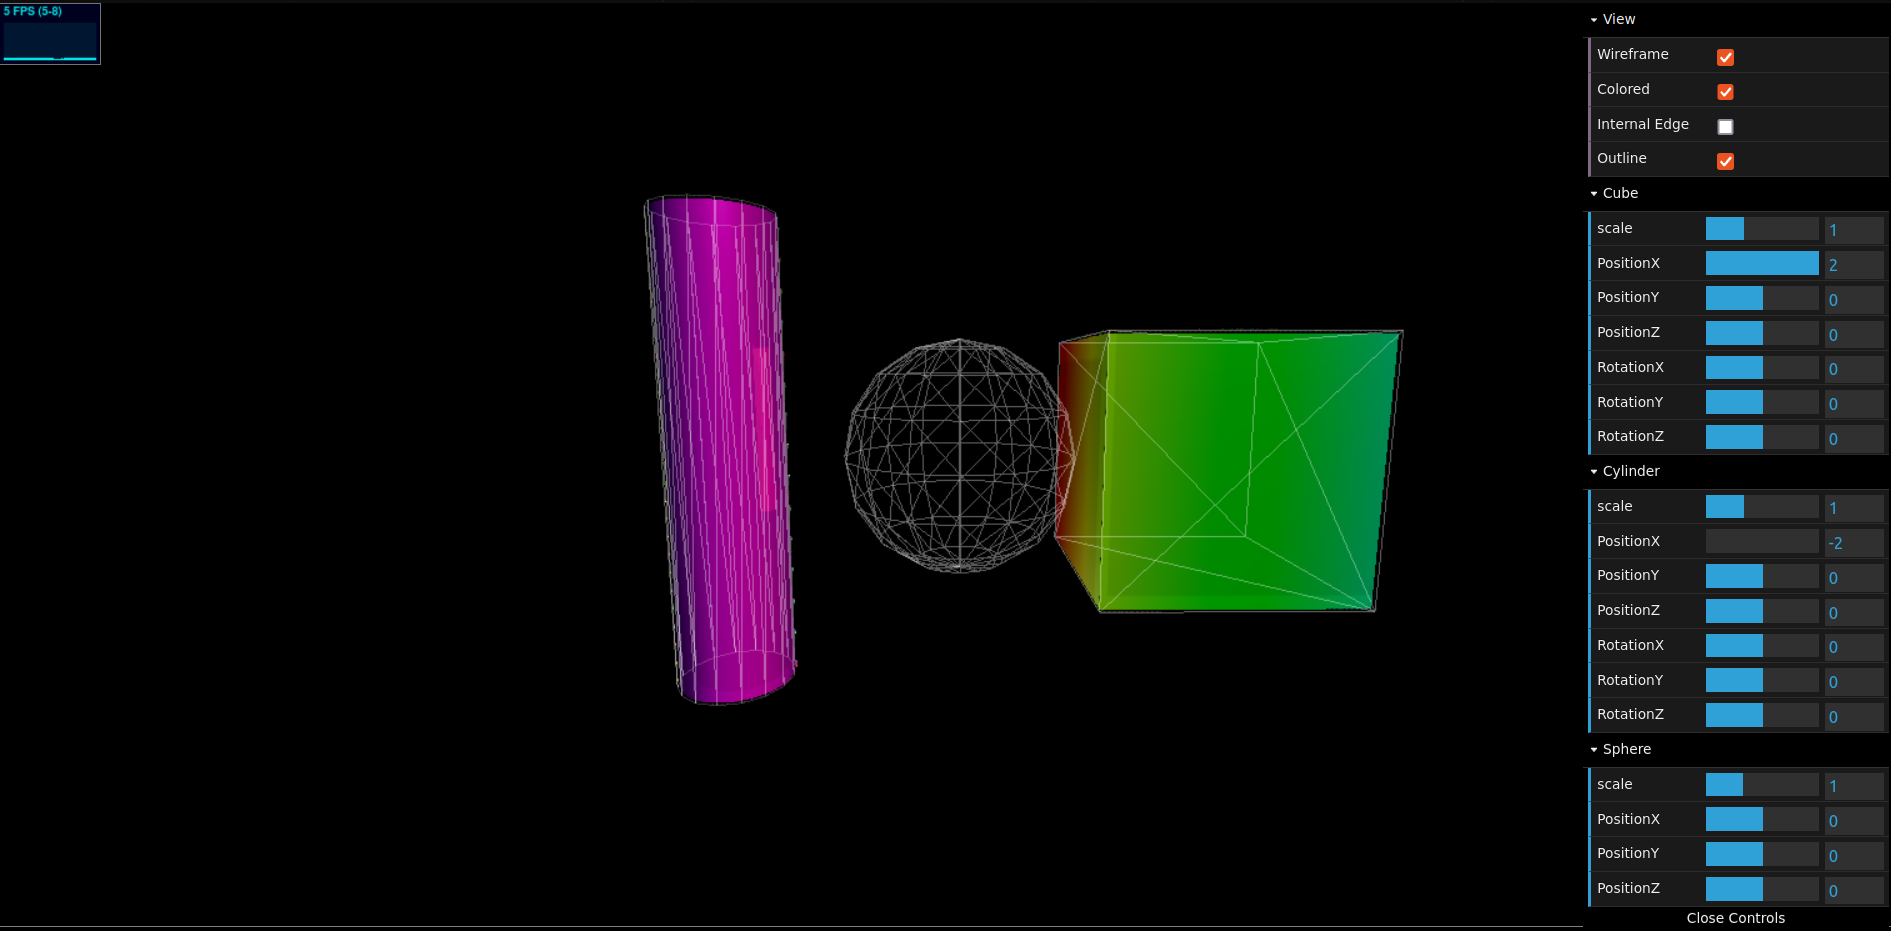
\includegraphics[scale=0.4]{inc/img/example_run}
  \caption{Демонстрация работы программы.}
  \label{fig:example_run}
\end{figure}

На сцене изображено три объекта (куб, сфера, цилиндр).
В настройках включен режим отображения каркаса, цветовая окраска.
\newpage
На рисунке \ref{fig:example_run_base} приведено изображение - композиция куба, 
сферы и цилиндра. 
На этом примере производится вычитание сферы из объединения куба и цилиндра.
\begin{figure}
  \centering
  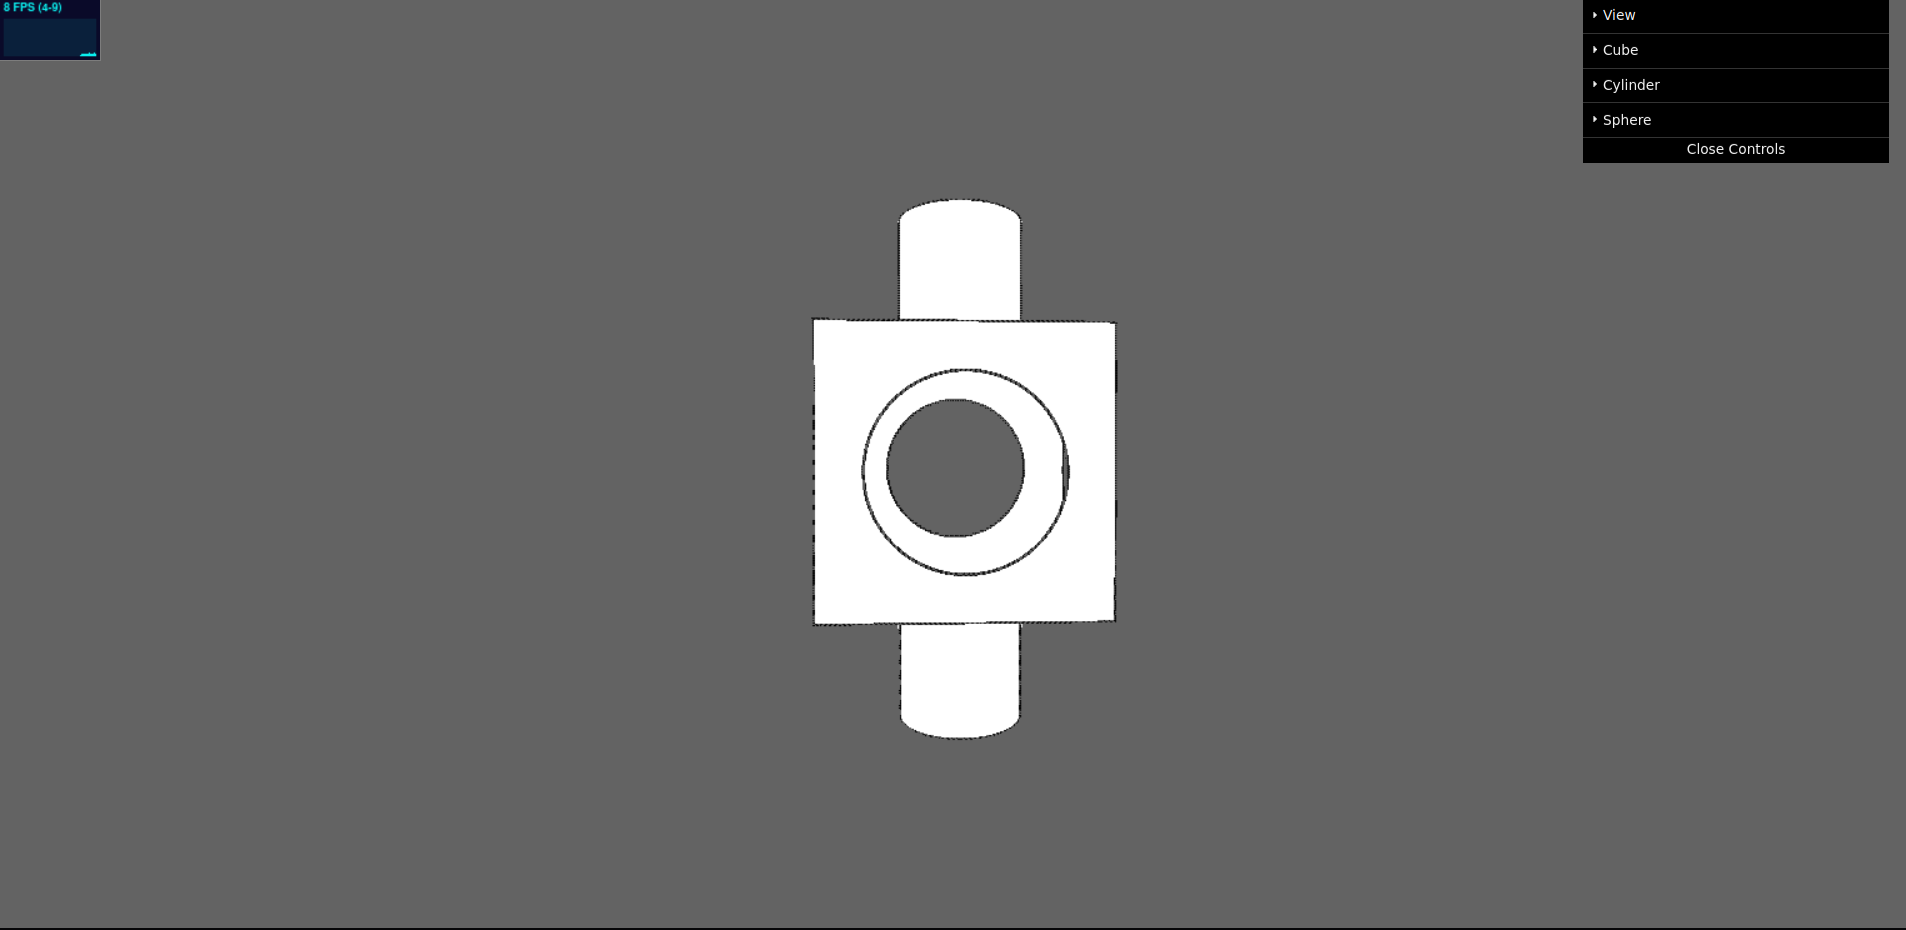
\includegraphics[scale=0.4]{inc/img/example_run_base}
  \caption{Демонстрация работы программы - композиция моделей.}
  \label{fig:example_run_base}
\end{figure}

\section{Постановка эксперимента}
\subsection{Цель эксперимента}

Целью эксперимента является сравнение производительности приложения при использовании встроенной и 
дискретной видеокарт.
Производительность будет оцениваться с помощью измерения количества кадров в секунду (FPS), с которами работает приложение.
Нагрузка будет меняться в зависимости от количества объектов, расположенных на сцене.  

\subsection{Технические характеристики}

Технические характеристики устройства, на котором выполнялось тестирование:

\begin{itemize}
	\item Операционная система: Ubuntu 21.04 \cite{ubuntu} Linux \cite{linux} 64-bit.
	\item Память: 19.4 GiB.
	\item Процессор: Intel Core™ i5-8300H \cite{intel} CPU @ 2.30GHz.
	\item Видеокарты: 
  \subitem Intel(R) UHD Graphics 630 (встроенная) \cite{intel-graphics}.
  \subitem NVIDIA GeForce GTX 1050 Mobile (дискретная) \cite{nvidia-gtx1050m}.
\end{itemize}
Тестирование проводилось на ноутбуке, включенном в сеть электропитания. Во время тестирования ноутбук был нагружен только системой тестирования (работающим приложением) и системным окружением операционной системы.

\subsection{Сравнение производительности}

Результаты сравнения производительности сцен разной нагруженности приведены в таблице \ref{tb:comp_fps}.
\begin{table}[]
  \caption{Сравнение FPS при запуске приложения на встроенной и дискретной видеокартах.}
  \begin{tabular}{|l|l|l|l|}
  \hline
  N & Количество объектов & FPS-NVIDIA & FPS-INTEL \\
  \hline
  1 & 1                   & 60         & 15        \\
  2 & 2                   & 60         & 12        \\
  3 & 3                   & 60         & 12        \\
  4 & 4                   & 58         & 10        \\
  5 & 5                   & 52         & 8         \\
  6 & 6                   & 41         & 8         \\
  7 & 7                   & 35         & 6         \\
  8 & 8                   & 23         & 5        \\
  \hline
  \end{tabular}
  \label{tb:comp_fps}
\end{table}

Результаты тестирования приводят к следующим выводам:
\begin{itemize}
  \item с ростом количества объектов, количество FPS уменьшается (в лучшем случае 60 кадров (23 на встроенной), в худшем 23 кадра (5 на встроенной));
  \item дискретная видеокарта позволяет получить большее количество кадров, которое приемлемо для использования приложения в режиме реального времени (30+ FPS),
  это объясняется наличием встроенной памяти (2 GB) и большей мощностью в сравнении с встроенной, которая менее производительна, а также использует разделяемую память (часть оперативной);
  \item встроенной видеокарты недостаточно для выполнения программы в режиме реального времени - приемлемое FPS должно быть около 30 и более, встроенная 
  (в лучшем случае - 1 объект на сцене) позволяет получить лишь 15 FPS -  для режима реального времени недостаточно;
  \item в среднем дискретная видеокарты производительнее встроенной в 4 раза;
  \item оптимальное количество одновременно отображаемых объектов находится в диапазоне от 1 до 7.
\end{itemize}


%%% Local Variables:
%%% mode: latex
%%% TeX-master: "rpz"
%%% End:
